%!TEX program = xelatex
\documentclass{beamer}
\RequirePackage{minted}
\RequirePackage{inputenc}

% Don't delete:
\newif\ifsplit
% It is necessary for switching from one outer theme to the other. By default, a miniframes outer theme is used for the header.
% Uncomment the following line to switch to a split outer theme:
\splittrue
% I suggest using the split outer theme if subsections are meaningful, miniframes otherwise.

\usetheme{Theme}

\title{compile-beamer}
\subtitle{with SciLifeLab template}
\author{MaxUlysse}
\institute{Barntumörbanken / SciLifeLab}
\date{2016/12/02}

\begin{document}

\begin{frame}[noframenumbering, plain]
	\titlepage
\end{frame}

\begin{frame}[fragile]
  \frametitle{compile-beamer}
  Just a simple beamer compiler with Nextflow
  Usage :
  \begin{minted}[fontsize=\tiny]{bash}
nextflow run MaxUlysse/compile-beamer \
  --tex <file.tex> \
  --theme <BTB||KI||SciLifeLab> \
  [--pictures <pictures directory>]
  \end{minted}
  This pdf was compiled using
  \begin{minted}[fontsize=\tiny]{bash}
nextflow run MaxUlysse/compile-beamer
  \end{minted}
\end{frame}

\begin{frame}[fragile]
  \frametitle{How to insert picture}
  \begin{minted}[fontsize=\tiny]{latex}
\begin{center}
  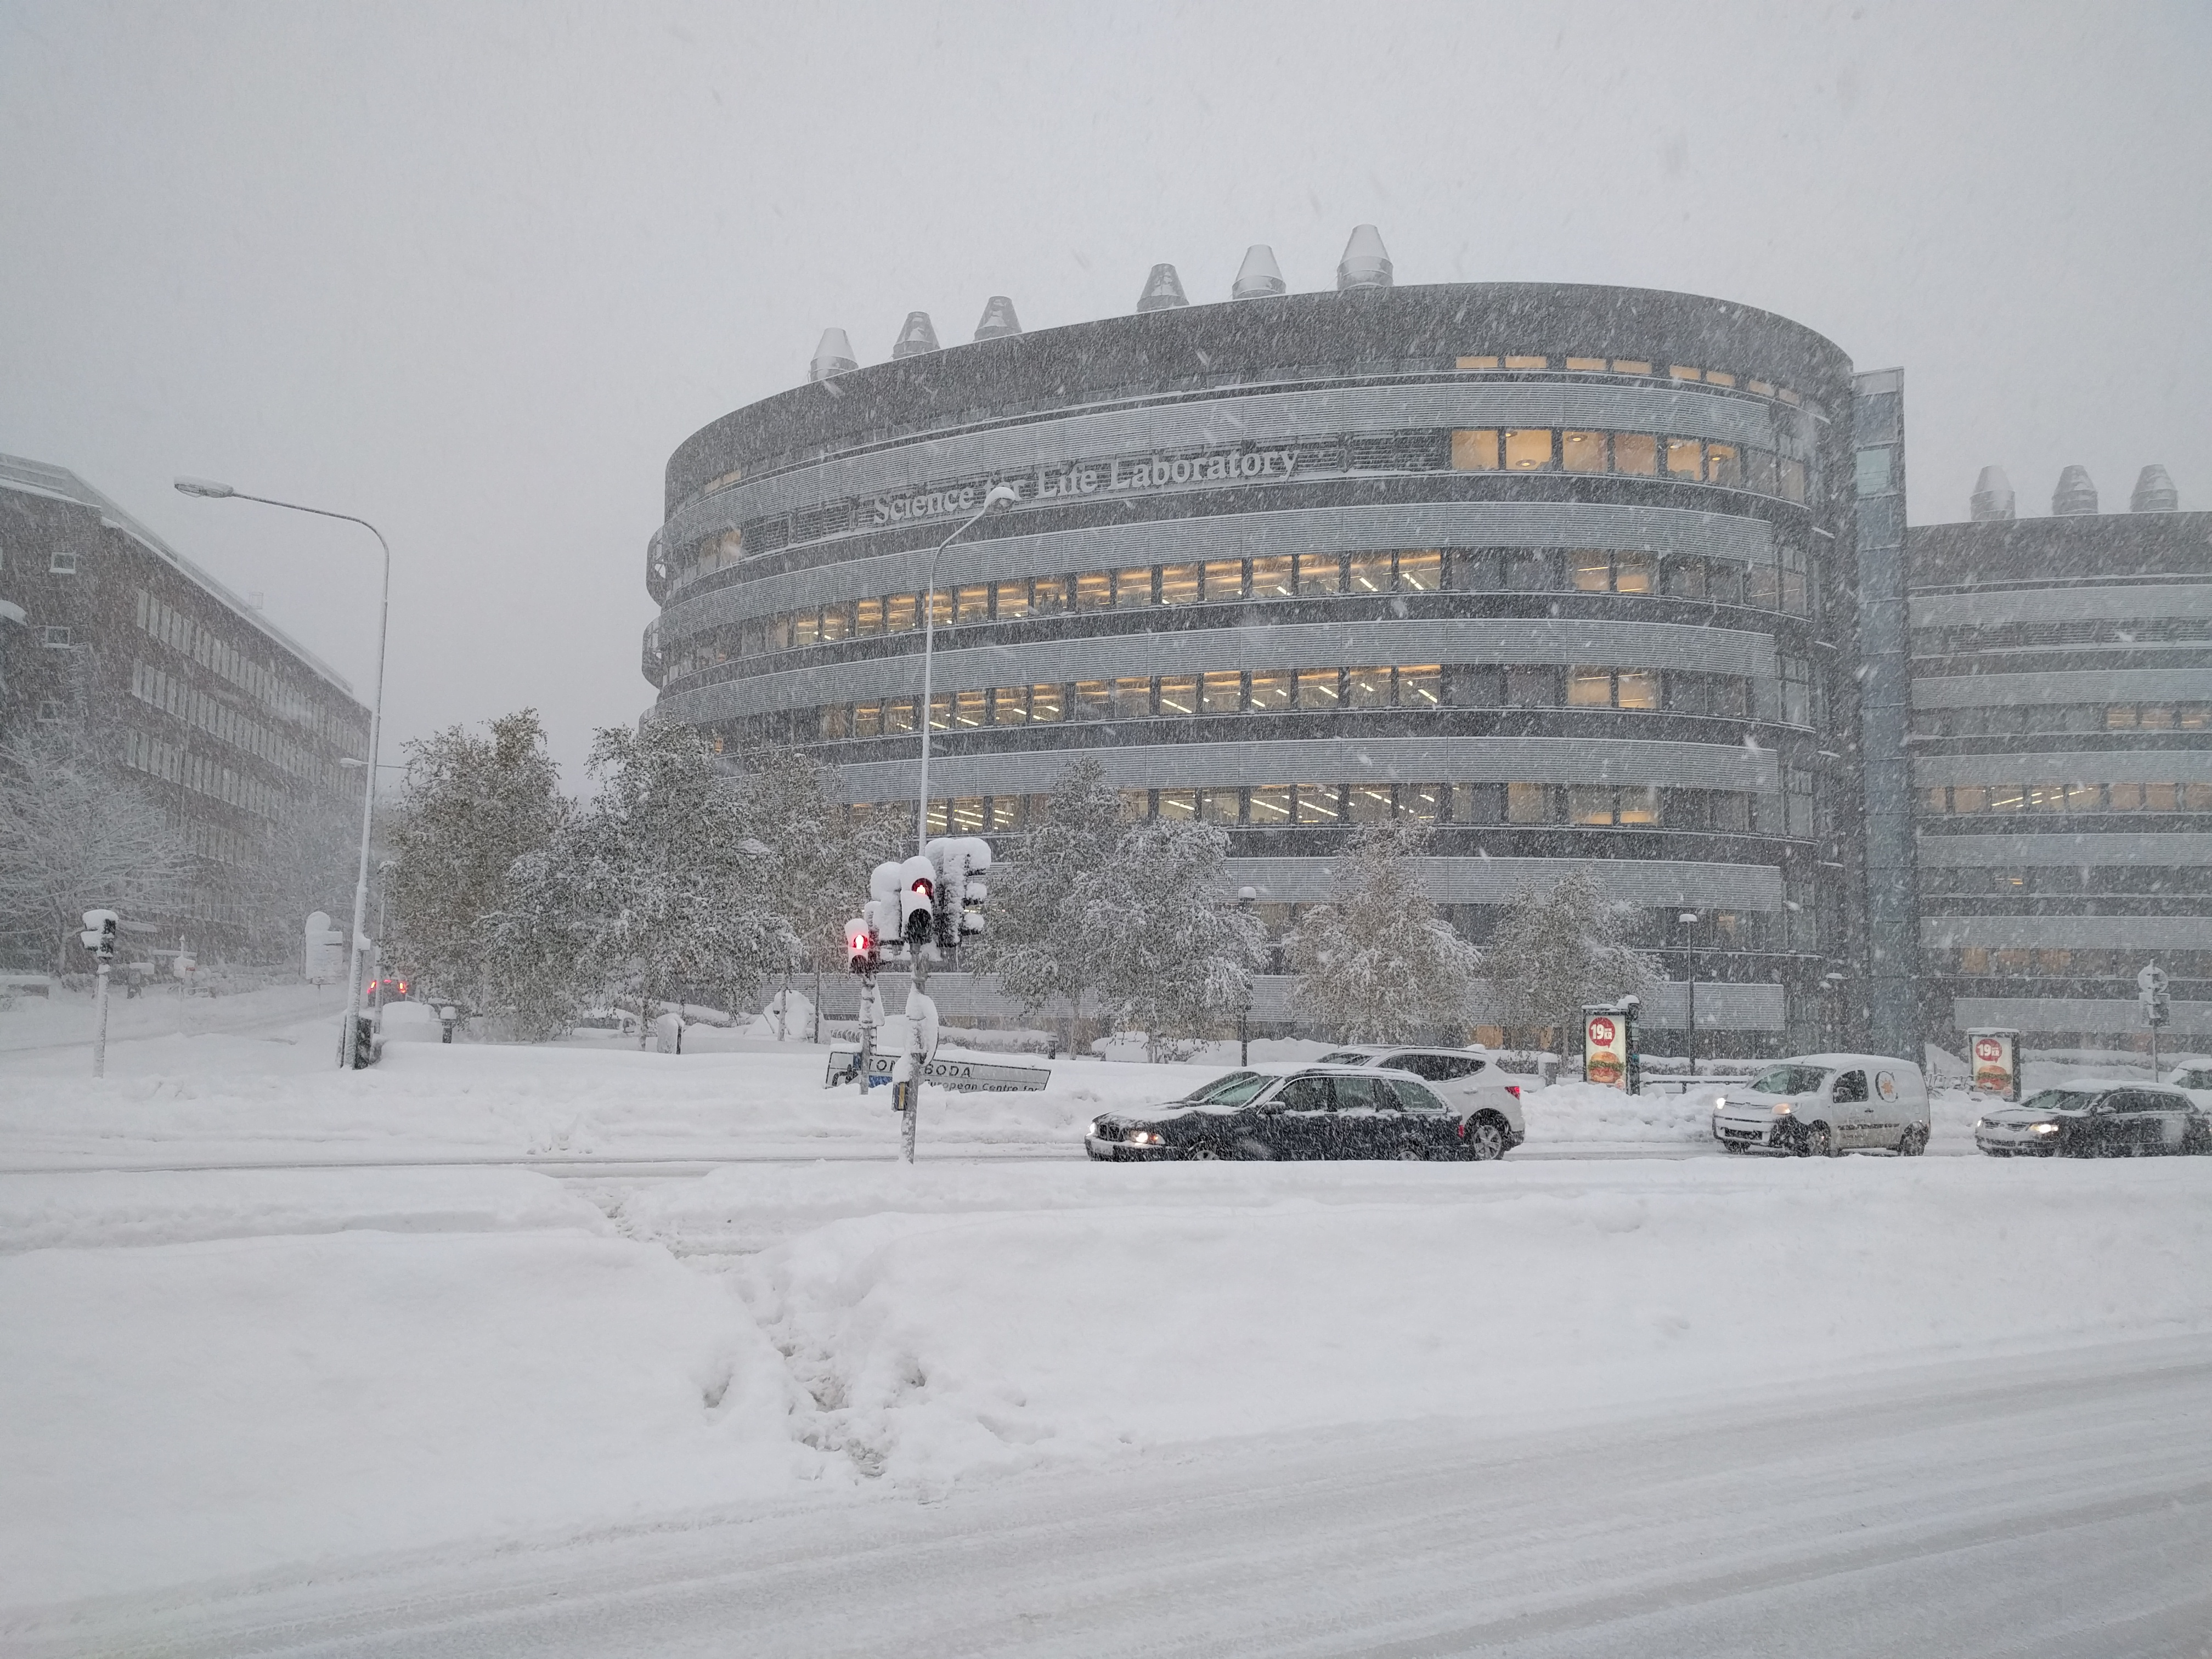
\includegraphics[width=.8\linewidth]{pictures/Snowpocalypse-SciLifeLab.jpg}
\end{center}
  \end{minted}
\end{frame}

\begin{frame}
  \frametitle{How to insert picture}
  \begin{center}
    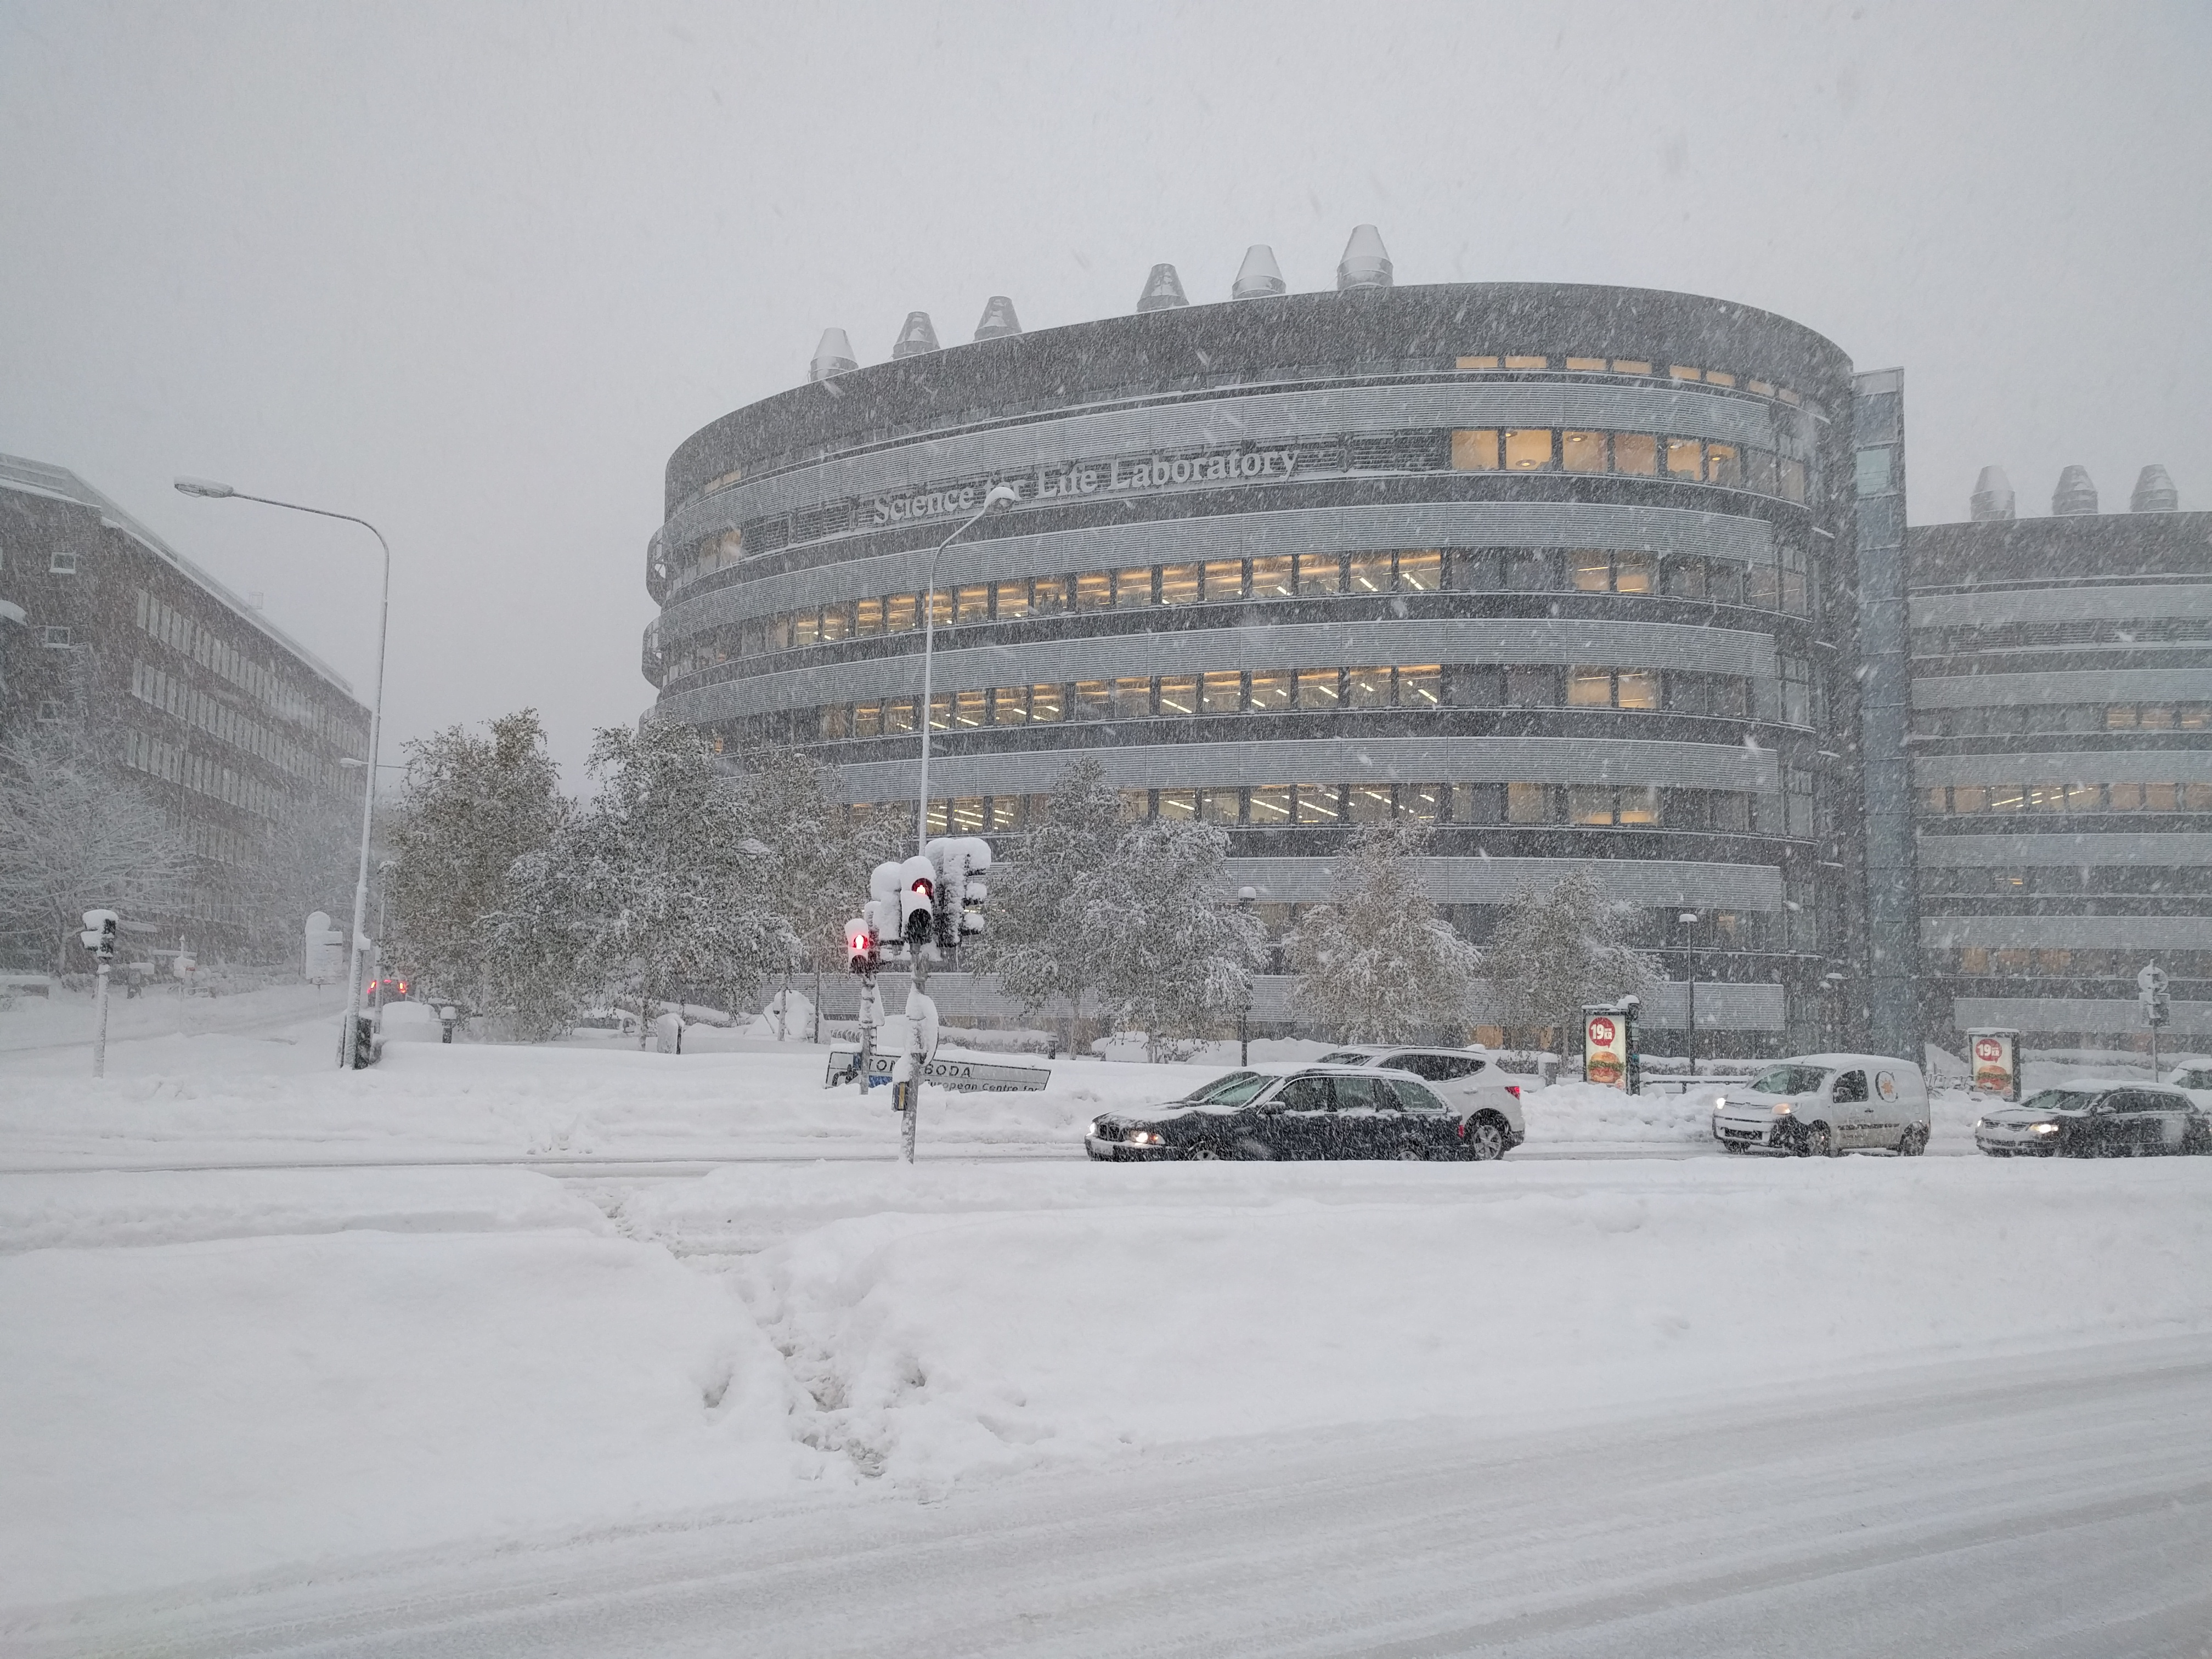
\includegraphics[width=.8\linewidth]{pictures/Snowpocalypse-SciLifeLab.jpg}
  \end{center}
\end{frame}

\end{document}
